\documentclass[11pt,a4paper]{article}
\usepackage[a4paper,margin=22mm]{geometry}
\usepackage{fontspec}
\usepackage{xeCJK}
\usepackage{amsmath}
\usepackage{booktabs}
\usepackage{longtable}
\usepackage{graphicx}
\usepackage{float}
\usepackage{xcolor}
\usepackage{hyperref}
\usepackage{array}
\usepackage{caption}

\setmainfont{Times New Roman}
\setsansfont{Arial}
\setmonofont{Consolas}
\setCJKmainfont{Yu Gothic}
\setCJKsansfont{Yu Gothic}
\hypersetup{colorlinks=true,linkcolor=blue,urlcolor=blue,citecolor=blue}
\captionsetup{font=small}

\newcommand{\pass}{\textcolor{green!45!black}{PASS}}
\newcommand{\fail}{\textcolor{red!70!black}{FAIL}}
\newcommand{\note}[1]{\par\smallskip\noindent\textbf{注:} #1\par\smallskip}

\title{CREE XHP70B-00-0000-0D0BN440E\\BWSC 2025 DRL光学検討・適合性監査報告書}
\author{drl-optical-sim audit report}
\date{2026-05-01}

\begin{document}
\maketitle

\begin{center}
\fcolorbox{red!60!black}{red!5}{
\begin{minipage}{0.92\linewidth}
\textbf{結論。} 現在保存されている \texttt{tests} のPASS結果は、20.3 mA駆動のCREE XHP70Bが実レンズでR148 category RLを満たした証拠ではない。\\
保存結果の入力光束は確かに約33.06 lmであり、20.3 mAで1710 lmを出す計算にはなっていない。しかし保存結果は \texttt{ideal\_r148\_1p756} による理想配光で、光度分布を規則表の1.756倍へ強制した検証モードである。したがって、実商品レンズの適合根拠としては使えない。
\end{minipage}}
\end{center}

\section{本報告書の範囲}
本報告書は、以下を確認するための技術監査である。

\begin{itemize}
\item 保存済みシミュレーション結果が、CREE XHP70B-00-0000-0D0BN440Eの20.3 mA運用を正しく扱っているか。
\item 見かけ面積の計算が単位換算として正しいか。
\item CREE XHP70B 1個を1灯体内に使う前提で、国内購入可能な実商品レンズだけでBWSC 2025 / UNECE R148 category RLを完全に示せるか。
\item 専門外の読者にも分かるように、規則要求、計算式、シミュレーションの裏側、保存画像の意味を説明すること。
\end{itemize}

\note{BWSC車両としては「two daytime running lamps」が必要である。ここでいう「1灯のみ」は、左右2個のDRLのうち片側1灯体を、LED 1個で構成するという意味で評価する。車両全体としては左右2灯が必要である。}

\section{参照資料}
\begin{longtable}{p{0.19\linewidth}p{0.74\linewidth}}
\toprule
資料 & 用途 \\
\midrule
BWSC 2025 Event Regulations Release Version 2.0 & Lighting条項2.23、audible warning条項2.24、glossaryのapparent surfaceを確認。\\
\url{https://cms.worldsolarchallenge.org/app/uploads/2024/12/3297_2025_bwsc_regulations_release_v20_published_28_october_2024.pdf} & \\
\addlinespace
UN Regulation No. 148 & DRL category RLの光度、見かけ面積、photometric requirementの根拠。\\
\url{https://unece.org/fileadmin/DAM/trans/main/wp29/wp29regs/2020/R148e.pdf} & \\
\addlinespace
Cree XLamp XHP70.2 data sheet & 型番、光束bin、12 V構成、FWHM、寸法、定格を確認。\\
\url{https://downloads.cree-led.com/files/ds/x/XLamp-XHP70.2.pdf} & \\
\addlinespace
エルパラ CREE XHP70/XHP70.2用オプティカルレンズ & 国内購入可能なXHP70/XHP70.2用レンズ候補。ページ上で光学特性データなしとされる。\\
\url{https://www.led-paradise.com/product/2600} & \\
\addlinespace
Carclo 10756 optics page & XHP70.2でFWHM、効率、cd/lmが公開されている比較対象。\\
\url{https://www.carclo-optics.com/optic-10756-led-cree-xlamp-xhp702-white} & \\
\addlinespace
Mouser Japan / LEDiL F15539\_JENNY-40 & 国内向けに購入可能な公開光学データ付きレンズ候補。\\
\url{https://www.mouser.jp/ProductDetail/Ledil/F15539_JENNY-40} & \\
\bottomrule
\end{longtable}

\section{BWSC 2025でDRLに関係する要求の抽出}
著作権上、規則本文の長文転載ではなく、条項番号と要求の要約として整理する。

\begin{longtable}{p{0.14\linewidth}p{0.80\linewidth}}
\toprule
条項 & 要求の要約 \\
\midrule
2.23.1 & 車両には左右2個のdaytime running lampを含む所定の灯火を装備する。\\
2.23.2 & DRLは白色でなければならない。自作灯体では色度要求への適合説明が必要。\\
2.23.3 & 灯体はUNECE R148またはSAE/DOT相当へ適合すること。適合マーク、またはcertifying engineerが確認した詳細なphotometric documentationが必要。lmからcdへの単純換算は不可。\\
2.23.4 & 正しい灯種を正しい位置・向きで取り付ける。DRLはUNECE category RL、SAE/DOT type Y2に対応する。\\
2.23.13 & DRLは前方に取り付ける。左右間隔、地上高、上下左右の幾何学的可視範囲を満たすこと。\\
2.23.16 & 走行可能状態ではDRLが動作すること。\\
2.24 & 車両全体としてはホーンも必要。DRL単体報告とは別に車両適合で確認が必要。\\
\bottomrule
\end{longtable}

\section{UNECE R148 category RL相当の数値要求}
本シミュレータに内蔵したR148 category RL相当の測定点は表\ref{tab:r148}である。各点でシミュレーション光度が最小値以上であること、最大光度が1200 cd以下であること、見かけ面積が25--200 cm\textsuperscript{2}であることを判定している。

\begin{table}[H]
\centering
\caption{R148 category RL相当の最小光度表 [cd]}
\label{tab:r148}
\begin{tabular}{c|rrrrrrr}
\toprule
$v\backslash h$ & -20 & -10 & -5 & 0 & +5 & +10 & +20\\
\midrule
+10 & 0 & 0 & 80 & 80 & 80 & 0 & 0\\
+5  & 40 & 80 & 180 & 280 & 180 & 80 & 40\\
0   & 100 & 280 & 360 & 400 & 360 & 280 & 100\\
-5  & 40 & 80 & 180 & 280 & 180 & 80 & 40\\
-10 & 0 & 0 & 80 & 80 & 80 & 0 & 0\\
\bottomrule
\end{tabular}
\end{table}

\section{CREE XHP70Bの20.3 mA運用条件}
登録したLEDデータは以下である。

\begin{itemize}
\item 型番: CREE LED XHP70B-00-0000-0D0BN440E
\item データシート上のbinning条件: 12 V構成、$I_F=1050$ mA
\item 光束bin: 1710 lm級
\item FWHM / 指向角: 125 deg
\item 点灯予定電流: 20.3 mA
\item 電力: $12.0\,\mathrm{V}\times0.0203\,\mathrm{A}=0.2436\,\mathrm{W}$
\end{itemize}

本シミュレータの初期電流換算は線形近似である。

\begin{align}
\Phi(I) &= \Phi_\mathrm{nom}\frac{I}{I_\mathrm{nom}}\\
        &= 1710\,\mathrm{lm}\times\frac{20.3\,\mathrm{mA}}{1050\,\mathrm{mA}}\\
        &= 33.06\,\mathrm{lm}
\end{align}

したがって、\textbf{20.3 mAで1710 lmが出る計算にはなっていない。}
保存済み \texttt{summary\_report.md} でも \texttt{Source flux: 33.060 lm} と出ている。

\section{保存済みPASS結果の監査}
\subsection{保存configの読み取り}
\texttt{E:\textbackslash drl-optical-sim\textbackslash tests\textbackslash simulation\_config.json} は以下の条件だった。

\begin{longtable}{p{0.38\linewidth}p{0.50\linewidth}}
\toprule
項目 & 値 \\
\midrule
LED & CREE XHP70B-00-0000-0D0BN440E\\
LED数 & 1\\
電流 & 20.3 mA\\
基準光束 & 1710 lm at 1050 mA\\
換算入力光束 & 33.06 lm\\
レンズ & \texttt{ideal\_r148\_1p756}\\
理想モード & true\\
理想光学効率 & 80 \%\\
見かけ面 & 60 mm $\times$ 45 mm\\
\bottomrule
\end{longtable}

\subsection{保存画像}
図\ref{fig:saved-ideal-heatmap}と図\ref{fig:saved-ideal-3d}は、保存済み結果の画像である。これらは「理想R148配光を表示したもの」であり、実レンズによる物理的ray tracing結果ではない。

\begin{figure}[H]
\centering
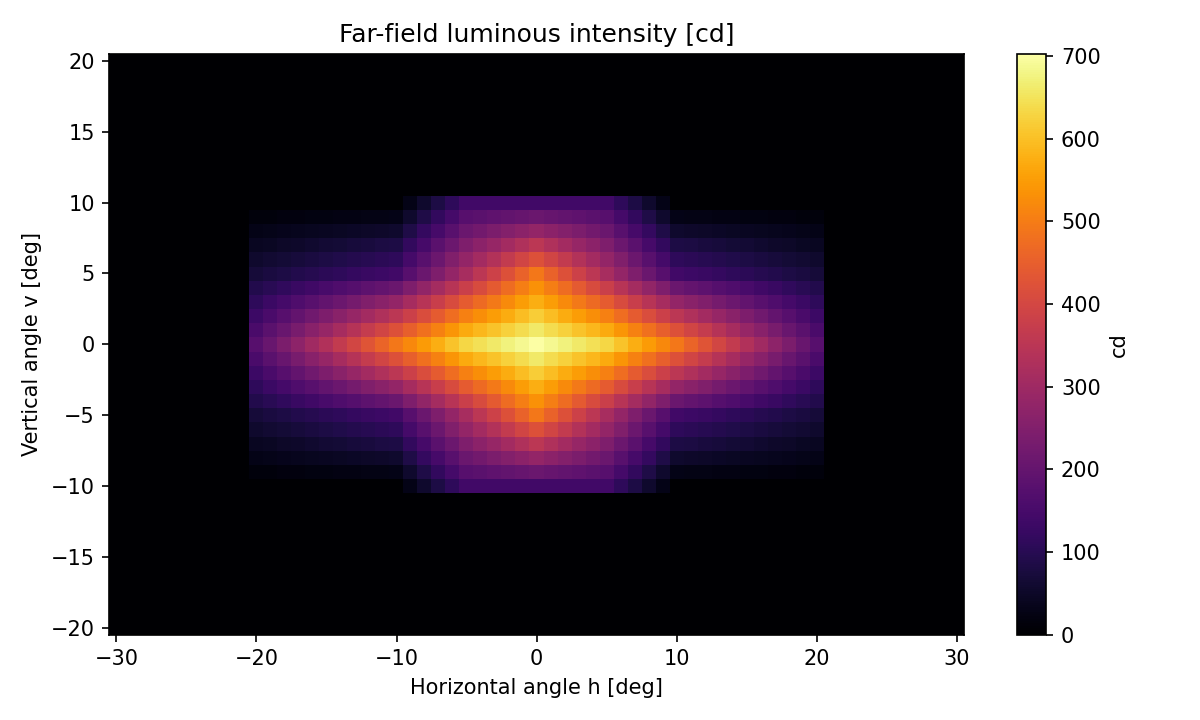
\includegraphics[width=0.90\linewidth]{figures/saved_ideal_heatmap.png}
\caption{保存済み理想モードの配光ヒートマップ。R148最小表の1.756倍へ強制した分布。}
\label{fig:saved-ideal-heatmap}
\end{figure}

\begin{figure}[H]
\centering
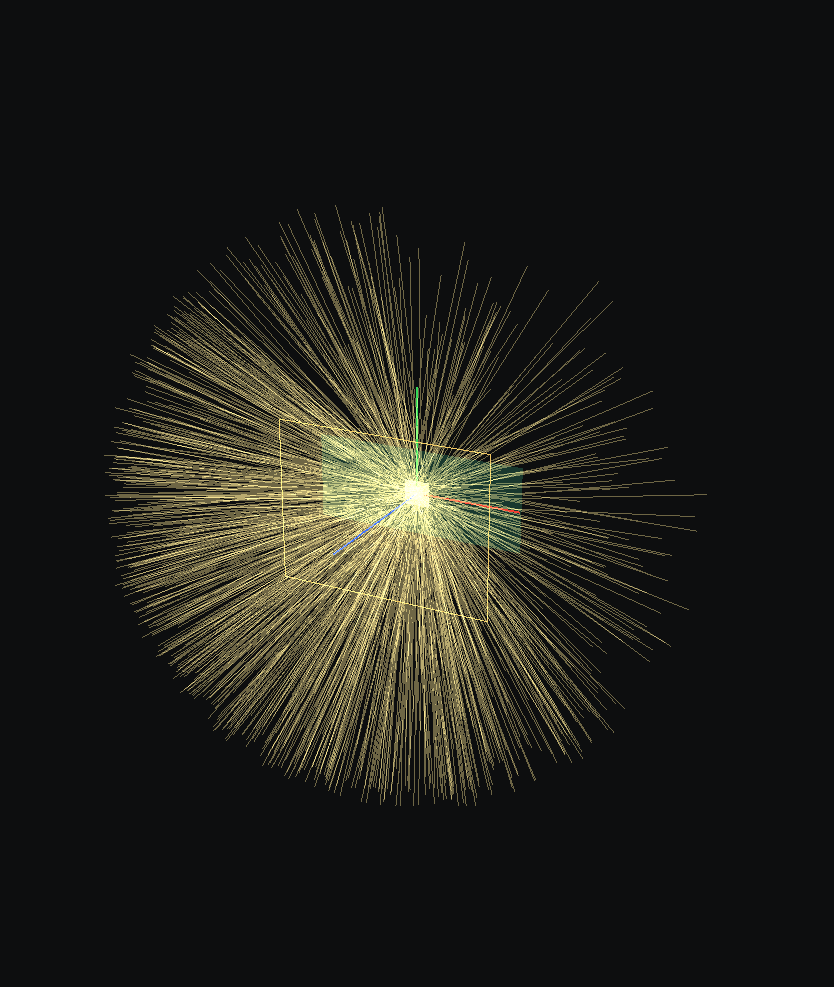
\includegraphics[width=0.72\linewidth]{figures/saved_ideal_3d_view.png}
\caption{保存済み3Dプレビュー。理想モードのため、これは実レンズの光路証明ではない。}
\label{fig:saved-ideal-3d}
\end{figure}

\subsection{なぜPASSが出たか}
理想モードでは、R148表の各測定点に対して

\begin{align}
I_\mathrm{ideal}(h,v)=1.756\,I_\mathrm{R148,min}(h,v)
\end{align}

を直接作る。そのため中心点は

\begin{align}
I(0,0)=1.756\times400=702.4\,\mathrm{cd}
\end{align}

となり、R148測定点は必ずPASSする。これは「目標配光を作った」だけであり、LED 33.06 lmと実レンズからその配光が得られたことを意味しない。

\subsection{エネルギー整合性}
保存条件では光学効率80 \%なので、出射光束は

\begin{align}
\Phi_\mathrm{exit}=33.06\times0.8=26.448\,\mathrm{lm}
\end{align}

である。一方、シミュレータの1 deg格子上でR148最小配光を補間して積分すると、以下になる。

\begin{longtable}{p{0.50\linewidth}r}
\toprule
分布 & 格子上の積分光束 \\
\midrule
R148最小相当、scale 1.000 & 33.44 lm\\
保存結果、scale 1.756 & 58.72 lm\\
保存結果の宣言出射光束 & 26.45 lm\\
\bottomrule
\end{longtable}

したがって保存PASS結果は、少なくとも現在の1 deg格子モデル上では光束収支と一致していない。これは意図的な検証モードの限界であり、実商品レンズの適合証明には使えない。

\section{実物理モデルでの確認: レンズなし}
同じLED、同じ20.3 mAで、理想モードを使わず、レンズなしのMonte Carlo ray tracingを行った。結果は表\ref{tab:nolens}である。

\begin{table}[H]
\centering
\caption{CREE XHP70B 1個、20.3 mA、レンズなしの物理計算}
\label{tab:nolens}
\begin{tabular}{lr}
\toprule
項目 & 値\\
\midrule
入力光束 & 33.06 lm\\
出射光束 & 33.06 lm\\
$I(0,0)$ & 9.23 cd\\
$I_\mathrm{max}$ & 18.78 cd\\
R148 RL判定 & \fail\\
\bottomrule
\end{tabular}
\end{table}

\begin{figure}[H]
\centering
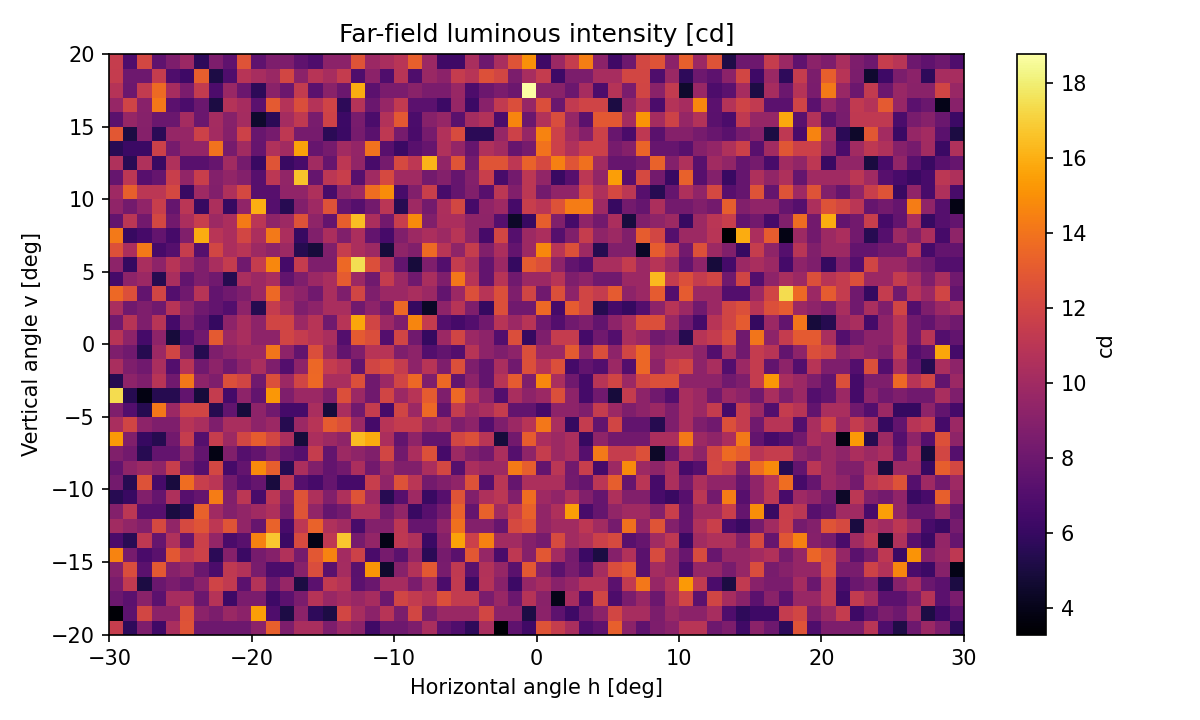
\includegraphics[width=0.90\linewidth]{figures/physical_nolens_heatmap.png}
\caption{レンズなし物理計算の配光。中心光度はR148 RLの400 cdに大きく不足する。}
\end{figure}

\section{見かけ面積の計算}
保存結果の見かけ面設定は60 mm $\times$ 45 mmである。矩形面として計算すれば、

\begin{align}
A &= \frac{60\,\mathrm{mm}\times45\,\mathrm{mm}}{100}\\
  &= 27.0\,\mathrm{cm^2}
\end{align}

であり、25--200 cm\textsuperscript{2}の範囲に入る。したがって\textbf{単位換算としては正しい}。

ただし、これは「その60 mm $\times$ 45 mm全体が完成灯体の見かけ発光面として認められる」ことが前提である。単にレンズ外径だけを見かけ面とするなら、たとえばエルパラのXHP70用レンズ外径32.42 mmでは、

\begin{align}
A_\mathrm{lens}=\pi\left(\frac{3.242\,\mathrm{cm}}{2}\right)^2=8.25\,\mathrm{cm^2}
\end{align}

となり、25 cm\textsuperscript{2}未満で不合格である。実車で合格させるには、25 cm\textsuperscript{2}以上に見える発光面、前面拡散板、または発光面定義を満たす灯体構造が必要である。

\section{最低条件の導出}
\subsection{中心光度だけで見たcd/lm要求}
R148 RL中心点の最小要求は400 cdである。20.3 mA時の入力光束33.06 lmから直接求めると、

\begin{align}
\frac{400\,\mathrm{cd}}{33.06\,\mathrm{lm}}=12.10\,\mathrm{cd/lm}
\end{align}

80 \%の光学効率を仮定し、出射光束26.448 lmで見ると、

\begin{align}
\frac{400\,\mathrm{cd}}{26.448\,\mathrm{lm}}=15.12\,\mathrm{cd/lm}
\end{align}

が必要である。保存済み理想モードの中心702.4 cdを20.3 mAで実現するなら、

\begin{align}
\frac{702.4\,\mathrm{cd}}{26.448\,\mathrm{lm}}=26.56\,\mathrm{cd/lm}
\end{align}

が必要である。

\subsection{中心光度だけでは不十分}
R148 RLは中心だけでなく、水平$\pm20^\circ$、垂直$\pm10^\circ$を含む複数点で光度を要求する。狭角レンズで中心400 cdだけを作っても、周辺測定点を満たせない可能性が高い。逆に広角レンズは周辺点を満たしやすいが、中心cd/lmが下がる。したがって必要なのは、単なるFWHMではなく、完成灯体の角度別光度表またはIES/LDT/実測配光である。

\section{国内購入可能な実商品レンズ調査}
2026-05-01時点で確認した候補を表\ref{tab:lenses}に示す。推定中心光度は20.3 mA、33.06 lmで、公開されているpeak intensity cd/lmをそのまま掛けた概算である。

\begin{longtable}{p{0.18\linewidth}p{0.18\linewidth}p{0.20\linewidth}p{0.14\linewidth}p{0.18\linewidth}}
\caption{実商品レンズ候補と20.3 mAでの中心光度見積り}
\label{tab:lenses}\\
\toprule
候補 & 国内購入性 & 公開光学データ & 中心光度概算 & 判定 \\
\midrule
\endfirsthead
\toprule
候補 & 国内購入性 & 公開光学データ & 中心光度概算 & 判定 \\
\midrule
\endhead
エルパラ LP-7070-29ZXS系 8/15/25/90/10x30 deg & 国内ショップで購入可能 & 商品ページに光学特性データなし & 不明 & 購入候補だが、計算証明に使えない。実測必須。\\
\addlinespace
Carclo 10756 & DigiKey等で国内発注可能な流通あり & XHP70.2、効率85 \%、FWHM 24 deg、3.7 cd/lm & $3.7\times33.06=122.3$ cd & 中心400 cdに不足。\\
\addlinespace
LEDiL F15539 JENNY-40 & Mouser Japanで在庫確認。 & XHP70.2、FWHM 42 deg、効率94 \%、1.7 cd/lm & 56.2 cd & 中心400 cdに不足。\\
\addlinespace
LEDiL C12868 FLARE-MAXI & Mouser系で取扱い。 & XHP70.2、105 x 28 deg、効率94 \%、1.1 cd/lm & 36.4 cd & 中心400 cdに不足。\\
\addlinespace
LEDiL C16371 HB-SQ-WWW & DigiKey等で取扱い。 & XHP70.2、約86 deg、効率85 \%、0.4 cd/lm & 13.2 cd & 中心400 cdに不足。\\
\bottomrule
\end{longtable}

\subsection{レンズ調査の結論}
\textbf{20.3 mA、CREE XHP70B 1個、国内購入可能な既製レンズのみ、公開データだけでBWSC/R148 category RLを完全に満たすと証明できる商品は見つからなかった。}

エルパラ品は国内で入手しやすいが、ページ上で光学データがないため、certifying engineerへ提出する計算根拠にはならない。CarcloやLEDiLのように公開cd/lmがある製品は、20.3 mAでは中心400 cdに届かない。狭角レンズなら中心光度を上げられる可能性はあるが、R148の$\pm20^\circ$や$\pm10^\circ$の測定点を満たす証明が別途必要になる。

\section{BWSC完全対応へ必要な次の証拠}
完全対応の根拠として提出できる形にするには、以下が必要である。

\begin{enumerate}
\item 左右2個のDRL灯体を車体上に配置した寸法図。左右間隔、地上高、外縁距離、可視角を記載する。
\item 完成灯体の見かけ発光面を25--200 cm\textsuperscript{2}にする設計図。
\item 完成灯体の実測配光。少なくともR148 RL測定点、最大光度、必要なfield内の低光度条件を含める。
\item 白色の色度測定。LED単体のCCTだけでなく、レンズ・拡散板後の完成灯体で確認する。
\item DRLが走行可能状態で点灯する制御説明と実機確認。
\item certifying engineerの確認。
\end{enumerate}

\section{最終判定}
\begin{center}
\fcolorbox{red!60!black}{red!5}{
\begin{minipage}{0.92\linewidth}
\textbf{現状判定: 完全適合証明としては不成立。}\\
保存済みPASS結果は理想配光モードの検証であり、CREE XHP70Bを20.3 mAで実商品レンズに通した結果ではない。入力光束は33.06 lmとして正しく換算されているが、理想モードの光度分布はその光束から物理的に導かれていない。見かけ面積は60 mm $\times$ 45 mmを実発光面として扱うなら27.0 cm\textsuperscript{2}で正しいが、実レンズ単体では不足する場合がある。\\
したがって、現時点で作れる正しい報告書は「完全適合証明」ではなく「ギャップ分析と実測計画書」である。
\end{minipage}}
\end{center}

\appendix
\section{保存ファイル}
\begin{itemize}
\item 理想モード保存結果: \texttt{E:\textbackslash drl-optical-sim\textbackslash tests}
\item 本監査報告書: \texttt{E:\textbackslash drl-optical-sim\textbackslash reports\textbackslash xhp70b\_drl\_audit}
\item レンズなし物理計算: \texttt{physical\_nolens} サブフォルダ
\end{itemize}

\section{注意表示}
高輝度LEDの直視は禁止である。XHP70B級のパワーLEDは低電流評価でも熱設計を省略してよい部品ではない。BWSC提出には、シミュレーションだけでなく、実測フォトメトリ、色度測定、取付図、certifying engineer確認が必要である。

\end{document}
